\section{Algorithm Explanation}

\subsection{Original Lévy Process}
The formula below is a subclass of the Lévy process, the introduction of relevant parameters is cited from the material \cite{Brownian} below.
$$
X_{t}=\mu t+\sigma B_{t}+\sum_{i=1}^{N_{t}} Y_{i}
$$

\begin{itemize}
    \item $\mu$ is called the linear drift of the process.
    \item $\sigma$ is called the Gaussian intensity of the process.
    \item $\left\{B_{t}\right\}_{t \geq 0}$ is a standard Brownian motion (that is, a continuous-time stochastic process with independent and stationary increments and with $B_{t} \sim N(0, t)$ for all $t \geq 0$ and $B_{0}=0$).
    \item $\left\{N_{t}\right\}$ is a Poisson process of intensity $\lambda \geq 0$ with inter-arrival times $T_{1}, T_{2}, T_{3}, ...$ (recall that $T_{i} \sim E x p(\lambda)$) and arrival times $S_{1}, S_{2}, S_{3}, ...$ (recall that $S_{n} = \sum_{i=1}^{n} T_{i}$).
    \item $Y_{1}, Y_{2}, Y_{3}$ is a sequence of independent and identically distributed random variables with distribution F. 
\end{itemize}
\vspace{0.2cm}


\subsection{Discrete Skeleton}
\subsubsection{Generation of Discrete Skeleton}
Simulation of $X_{t}$ consists simulating the Brownian motion, of which process is generally difficult and inefficient. Hence, a discrete ``skeleton”\cite{Brownian} of $
\left\{X_{t}\right\}_{t \geq 0}\left(\operatorname{say}\left\{\left(P_{i}, A_{i}, M_{i}\right)\right\}_{i \in \mathbb{N}}\right.$, a 3-coordinate discrete stochastic process) is introduced to transform the simulation of continuous process to discrete one. 
\begin{itemize}
    \item $P_{i}$ is equal to $X_{S_{i}^{-}}$, that is, equal to the process $\left\{X_{t}\right\}_{t \geq 0}$ prior to its i-th jump.
    \item $A_{i}$ is equal to $X_{S_{i}}$, that is, equal to the process $\left\{X_{t}\right\}_{t \geq 0}$ after its i-th jump.
    \item $M_{i}$ is equal to $\sup _{0 \leq s \leq S_{i}} X_{s}$, that is, the maximum of $\left\{X_{t}\right\}_{t \geq 0}$ up to the time of its i-th jump.

\end{itemize}

With the discrete skeleton, one is able to describe the ${X}_t$ at the time point ${S}_i$ (i.e. the moment can be interpreted either before or after the jump.) However, the continuous process between ${X}_t$ corresponding to the Brownian motion can not be illustrated in this way.



\subsubsection{Principle of Discrete Skeleton}
1. Theorem\cite{Brownian}:
\begin{itemize}
    \item Assume $ T \sim E x p(\lambda)$.
    \item $ V=\max _{0 \leq t \leq T} \mu t+\sigma B_{t}$, where $V_{i}$ will be the highest point that $\left\{\mu t+\sigma B_{t}\right\}_{t \geq 0}$ reaches before the next inter-arrival time $T_{i}$.
    \item $W=\left(\max _{0 \leq t \leq T} \mu t+\sigma B_{t}\right)-\left(\mu T+\sigma B_{T}\right)$, where ${W}_{i}$ will be the point whose value equals to $V_{i}$ minus the value at time $T_{i}$.
    \item $V \sim E x p\left(\phi_{1}\right)$, where
    $\phi_{1}=-\frac{\mu}{\sigma^{2}}+\sqrt{\frac{\mu^{2}}{\sigma^{4}}+\frac{2 \lambda}{\sigma^{2}}}$
    \item $W \sim E x p\left(\phi_{2}\right)$, where 
    $\phi_{2}=\frac{\mu}{\sigma^{2}}+\sqrt{\frac{\mu^{2}}{\sigma^{4}}+\frac{2 \lambda}{\sigma^{2}}}$
\end{itemize}

2. Induction:
\begin{enumerate}
    \item[(1)] $T \sim E x p(\lambda)$, which means
    the linear drift and Brownian motion continuously take place during the time interval $T_{i-1}$ before the i-th jump occurring at the point $S_{i}$
    \item[(2)] $V$ and $W$ follow the exponential distribution with different rate, it is simple to simulate $V_{i}$ and $W_{i}$. Apparently, $V_{i}-W_{i} = \mu T_{i}+\sigma B_{{T}_{i}}$, then it is easy to obtain the value of the process at time $T_{i}$, which is $V_{i}-W_{i}$ (i.e. the combination of linear drift and Brownian motion during $T_{i}$);
    \item[(3)] Simulate $Y_{i}$ following the specific distribution F with corresponding parameters, where $Y_{i}$ means the size of i-th jump;
    \item[(4)] From the illustration before, the discrete ``skeleton'' of $\left\{X_{t}\right\}_{t \geq 0}$ can be expressed as:
    
    \begin{figure}[H]
    \centering
    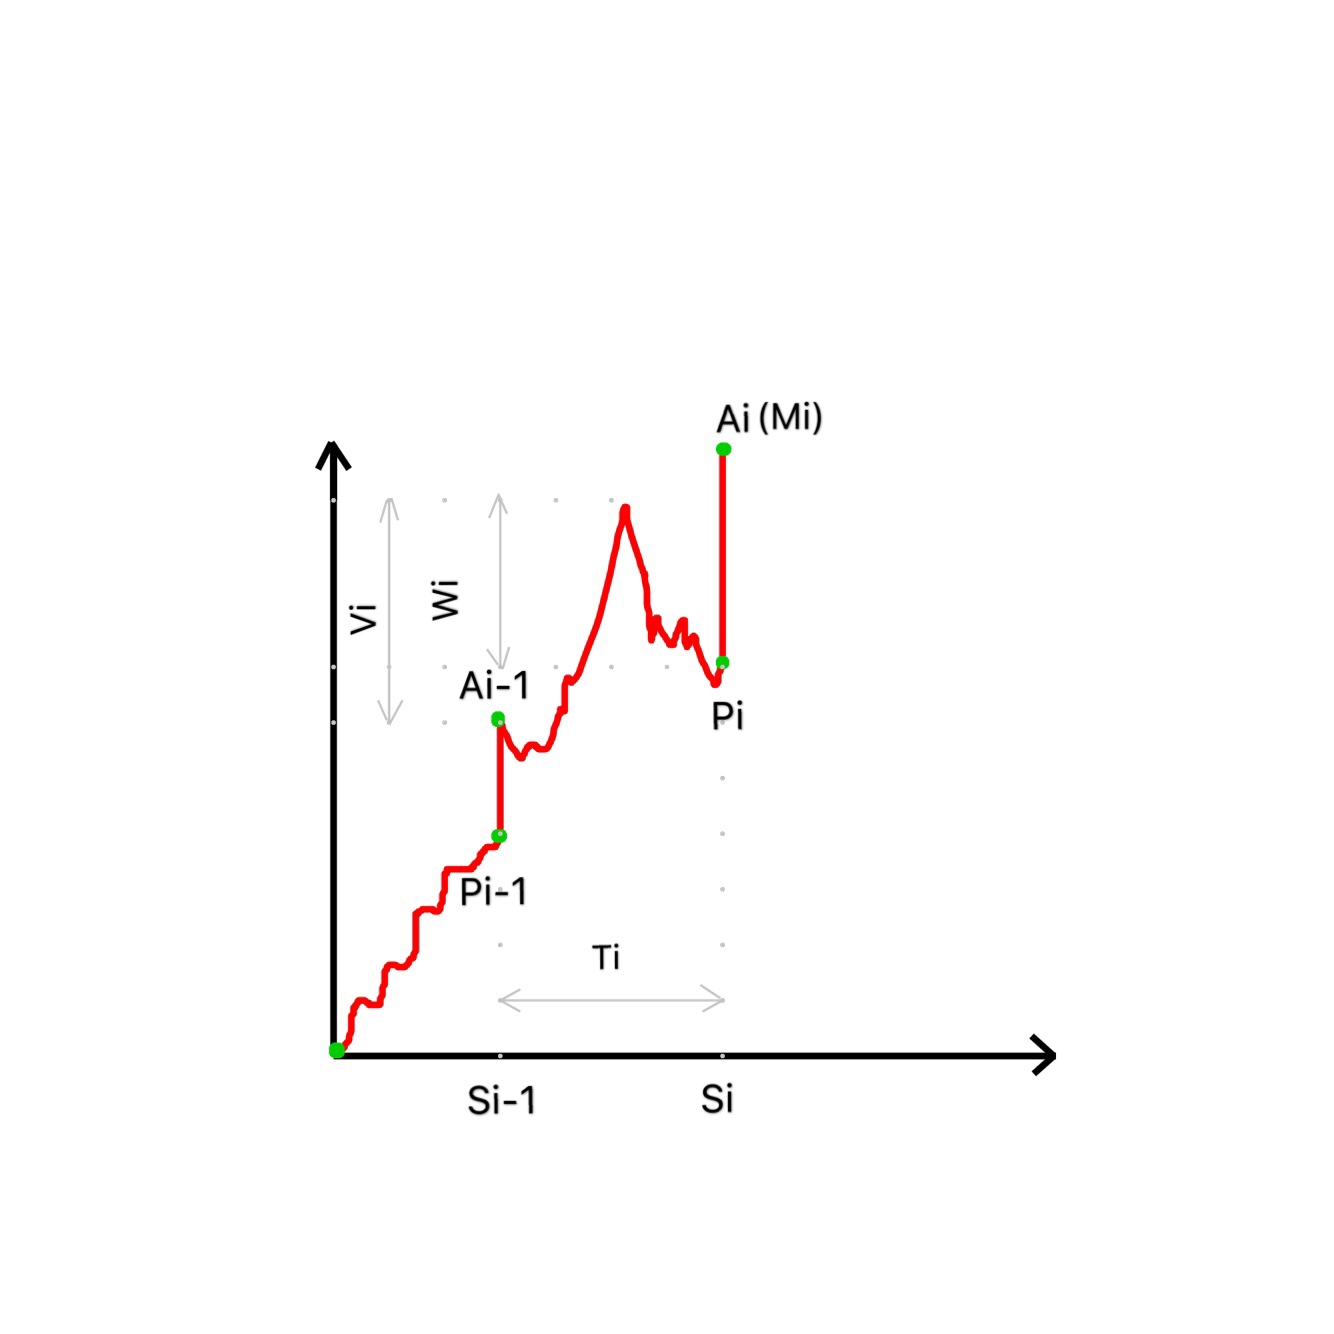
\includegraphics[scale=0.25]{figures/Illustration.png}
    \caption{Illustration}
    \label{fig:my_label}
\end{figure}
    
    \begin{itemize}
        \item $P_{i}=A_{i-1}+\left(V_{i}-W_{i}\right)$, which means $P_{i}$ equals to the sum of:\\
        a. The value of the former point $A_{i-1}$ which is obtained after (i-1)-th jump;\\
        b. The value of the process $\mu T_{i}+\sigma B_{{T}_{i}}$.
        
        \item $A_{i}=A_{i-1}+\left(V_{i}-W_{i}\right)+Y_{i}$, which means $A_{i}$ equals to $P_{i}+Y_{i}$ (i.e. the value of $P_{i}$ plus the size of i-th jump).
        
        \item $M_{i}=\max \left\{M_{i-1}, A_{i-1}+V_{i}, A_{i-1}+\left(V_{i}-W_{i}\right)+Y_{i}\right\}$, which means $M_{i}$ equals to the maximum value of all the points in time period [0, $S_i$].  
    \end{itemize}{}
    
\end{enumerate}{}







\newpage


